%%
%% Author: jamie
%% 05/10/18
%%
\chapter{Agent Implementation}\label{ch:development}

\section{UCT Algorithm}\label{sec:MCTS}

\subsection{Tree Representation}\label{subsec:treeRepresentation}

\subsection{UCB Selection}\label{subsec:selection}

\subsection{Expansion}\label{subsec:expansion}

\subsection{Simulation}\label{subsec:simulation}

\subsection{Tree Update}\label{subsec:treeUpdate}

\subsection{Smooth UCT}\label{subsec:smoothUCT}

\section{Best Response Computation}\label{sec:bestResponseComputation}
In order to evaluate the performance of our agent we utilised exploitability as our primary metric.
Exploitability is a measure of how well our agent would fare against an opponent responding
optimally to our strategy.
Exploitability is related to the concept of Nash equilibria in that a Nash equilibrium
is induced by a strategy that cannot be exploited.

To calculate the exploitability of a strategy we must determine the best responses
to that strategy.
The first step in calculating the best response strategy involves
taking our agent's action selections and inserting them into the game tree\citep{heinrich2017reinforcement}.
In other words, wherever the agent must take an action in the game tree, we choose the best action
based on our MCTS estimations.
As such the resultant tree will consist of the MCTS player's decision nodes which will have
a single child node along with the second player's decision nodes and chance nodes
which will both have multiple children.
We can then evaluate the terminal states and propagate values back up the tree, with the highest
child value being propagated when we reach a decision node for player two and the average child
value being propagated for chance nodes.
This process will now be explained in detail with coding examples.

\subsection{Generating Best Response Tree}\label{subsec:applyMCTS}

\begin{figure}[ht]
    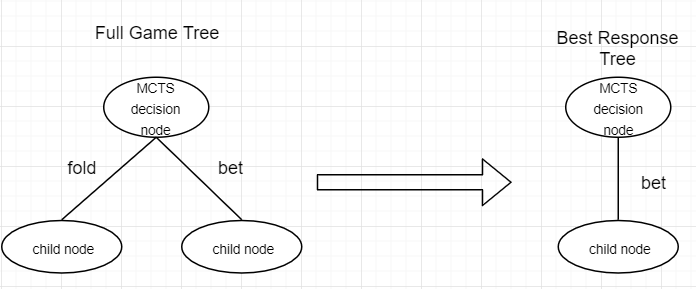
\includegraphics[scale=1]{images/best_response_tree_vs_full_tree.PNG}
    \caption{Generation of Best Response Tree}
\end{figure}

\subsection{Propagating Terminal Values}\label{subsec:propagateTerminals}
\subsection{Exploitability}\label{subsec:exploitability}

\section{Prototype Application}\label{sec:prototypeApp}
In order to give visual evidence of the work done and the agent developed, a user interface(UI) was created
that allowed human interaction with the trained bot.
In order to facilitate the development of this interface in a short period of time the Qt framework was used.
Qt is a open-source widget toolkit for creating graphical user interfaces and applications.
Specifically Qt Designer was used in order to generate a UI template.
Qt Designer is a what-you-see-is-what-you-get (WYSIWYG) UI generation tool that accompanies Qt.
PyQt5 was then used to generate python code from this UI template and connect the functional component of the game.
In this section we will briefly outline the process involved in creating this prototype application
and highlight some key code snippets.

In order to elicit requirements for this application I applied brainstorming as well as analysing a number
of online UIs that served a similar purpose to mine.
This process rendered the following functional requirements:
\begin{itemize}
    \item Display list of available actions.
    \item Allow user to take action.
    \item Display relevant cards to player.
    \item Annotate the sequence of events that occur in the game.
    \item Display the current pot size.
    \item Allow player to play multiple rounds.
    \item Keep track of cumulative winnings across multiple rounds.
\end{itemize}

\subsection{UI Screen}\label{subsec:UiScreen}
The first step towards achieving these functional requirements was to generate a UI screen.
This was achieved through Qt designer using drag and drop with the end result being as shown below.

\begin{figure}[ht]
    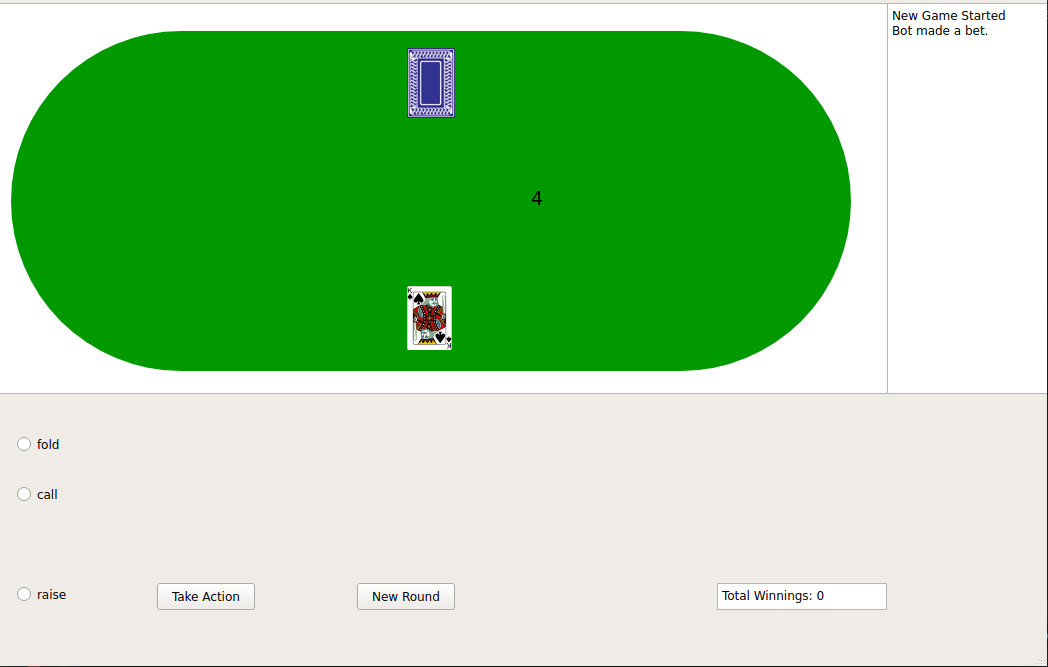
\includegraphics[scale=.4]{images/UI_screenshot.png}
    \caption{Game UI}
\end{figure}

\subsection{Event Handling and UI Manipulation}\label{subsec:eventHandling}


\subsection{Game Model}\label{subsec:gameModel}

\subsection{Agent Representation}\label{subsec:agent}

\begin{lstlisting}[style=Python]
    class Agent:
        def __init__(self, strategy_file):
            self.strategy = self.load_strategy(strategy_file)
\end{lstlisting}

